\section{Grundlagen}\label{sec:Grundlagen}
In diesem Kapitel wird der grundlegende Ablauf des Schleppvorgang beschrieben und die Funktion der beiden Windentypen (Einzug- und Abrollwinde) genauer beschrieben. Weiter sind die für dieses Projekt grundlegenden Anforderungen aufgelistet, wobei eine detaillierte Übersicht im Anhang \ref{appsec:Anforderungen} ersichtlich ist.

%für den Bericht grundlegende Informationen beschrieben. Diese werden zum einen in Richtlinien unterteilt,welche hauptsächlich aus den gesetzlichen Bestimmungen bestehen. Zum anderen ist ein mathematischer Teil vorhanden, wobei die Berechnungen mathematische Formeln aufweisen auf welche in den nachfolgenden Kapiteln verwiesen wird. 


\subsection{Schleppvorgang}\label{subsec:Schleppvorgang}
Der Gleitsegelschleppvorgang kann trotz zwei unterschiedlichen Ausführungen (Einzug- und Abrollwinde) mit demselben Prinzip beschreiben. Der Pilot steht startbereit am Boden und ist über auslösbare Verbindungen an ein Seil angemacht. Sobald der Schleppvorgang startet, wird das Seil zwischen Winde und Pilot gestraft bis er eine Kraft in horizontaler Richtung erfährt. Er beginnt zu rennen, wobei sich der Schirm über ihm aufrichtet. Sobald der Pilot eine genügend hohe Geschwindigkeit in Horizontalrichtung hat (in Bezug zum Wind), erfährt er eine Geschwindigkeit in Vertikalrichtung und hebt ab. Die dafür notwendige horizontal Geschwindigkeit ist abhängig vom Schirmtyp. Ein typischer Startvorgang ist in nachfolgender Abbildung \ref{fig:Sicherheitsstart} gut ersichtlich. Es gilt zu erwähnen, dass der ersichtliche Schleppvorgang bei einem Gegenwind von 5m/s abgebildet ist. Bei einer Vorwärtsgeschwindigkeit von 5m/s erreicht somit der Pilot eine Horizontalgeschwindigkeit von 10m/s gegenüber Wind.

\begin{figure}[H]
	\begin{center}
		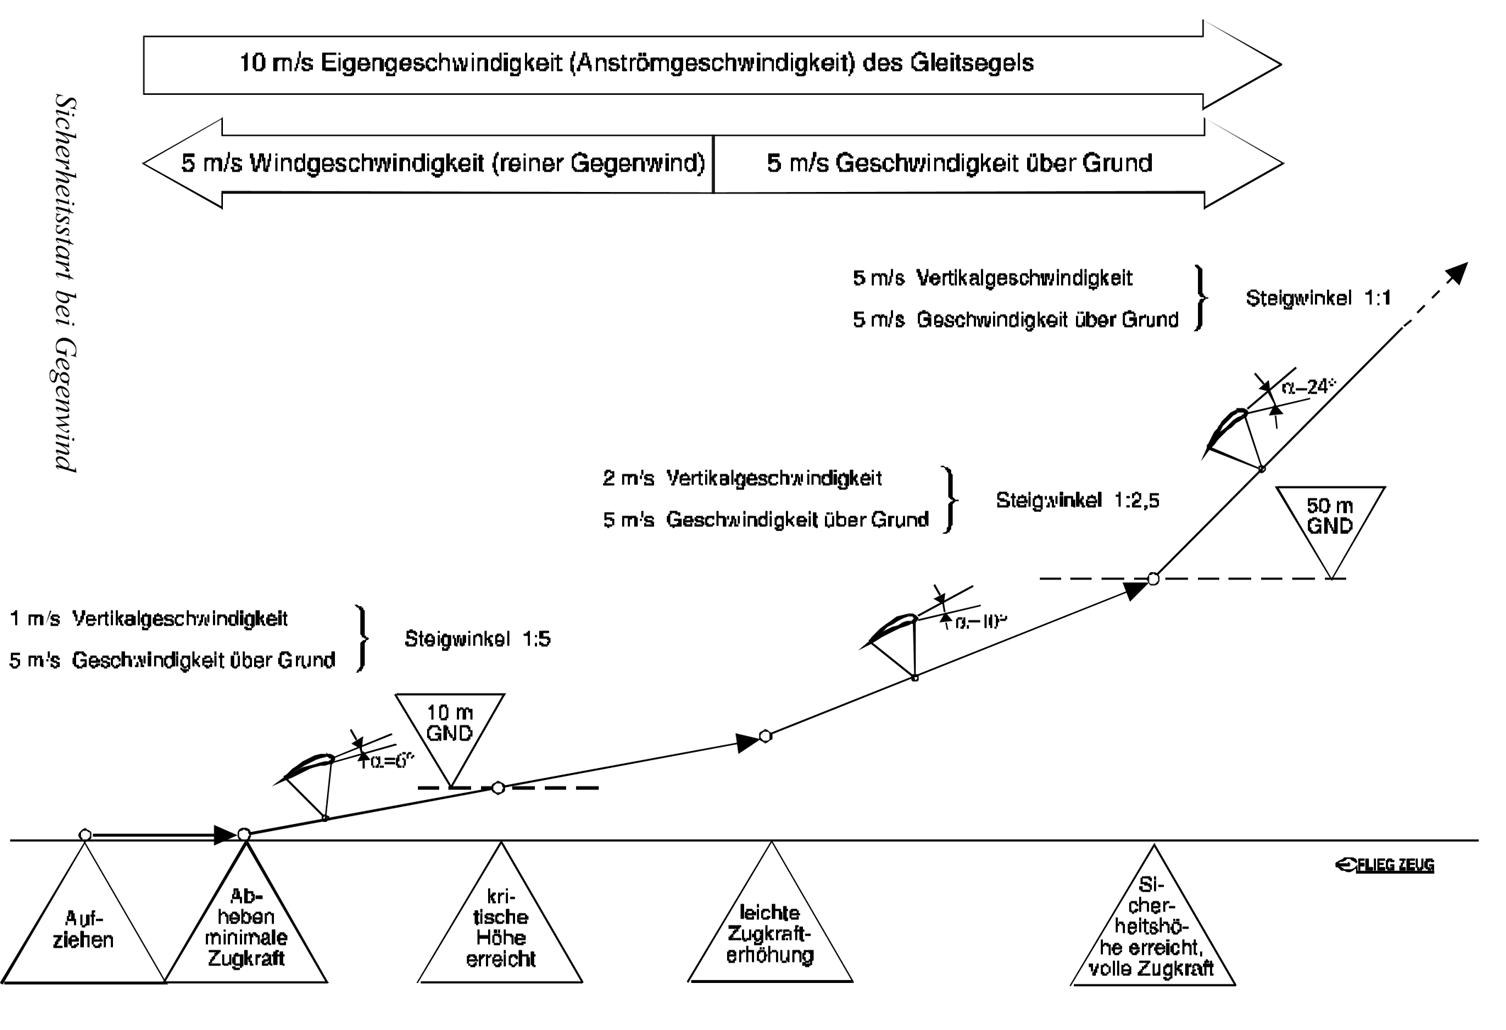
\includegraphics[width=160mm]{Sicherheitsstart.png}
		\caption{Sicherheitsstart beim Schleppvorgang \cite{Gleitsegelschlepp}}
		\label{fig:Sicherheitsstart}
	\end{center}
\end{figure}

In Abbildung \ref{fig:Sicherheitsstart} ist gut ersichtlich, dass der Startvorgang in vier Bereiche unterteilt wird. Die erste Phase beinhaltet die Seilstraffung bis zum Zeitpunkt des Abheben des Piloten. Der zweite Bereich umfasst die kritischste Phase, da der Pilot nur eine geringe Distanz zum Boden vorweist und bei einem Trennvorgang schnell reagieren muss. Damit ein unvorhergesehener Trennvorgang vom Piloten kontrolliert werden kann, darf die Zugkraft am Seil 30\% der Nennzugkraft nicht überschreiten. Sobald eine Höhe von 20m erreicht wurde, wird der Zug des Seils auf 70\% der eingestellten Nennzugkraft erhöht. Ab einer Höhe von 50m kann auf 100\% erhöht werden wodurch der Pilot mit einem Winkel (gegenüber Grund) von rund $22^\circ$ steigt. Diese Phase hält solange an, bis der Pilot die gewünschte Höhe erreicht hat oder mangels Seillänge der Vorgang beendet werden muss. Die Zugkraft wird erneut reduziert, so dass der Zug am Piloten abnimmt und der Schirm sich wieder über den Piloten neigt. Bei einer Zugkraft von wiederum 30\% der Nennzugkraft trennt sich nach Zeichenabsprache mit dem Windenführer der Pilot vom Seil. Diese Flugkurve mit den entsprechenden Steigwinkeln des Piloten gegenüber Grund ($\beta$) und dem Winkel des Seils ($\gamma$) ist in nachfolgender Abbildung \ref{fig:HoehenverlaufSchlepp} ersichtlich. Hier wird anders als bei der Abbildung \ref{fig:Sicherheitsstart} der Pilot von rechts nach links gezogen.


\begin{figure}[H]
	\begin{center}
		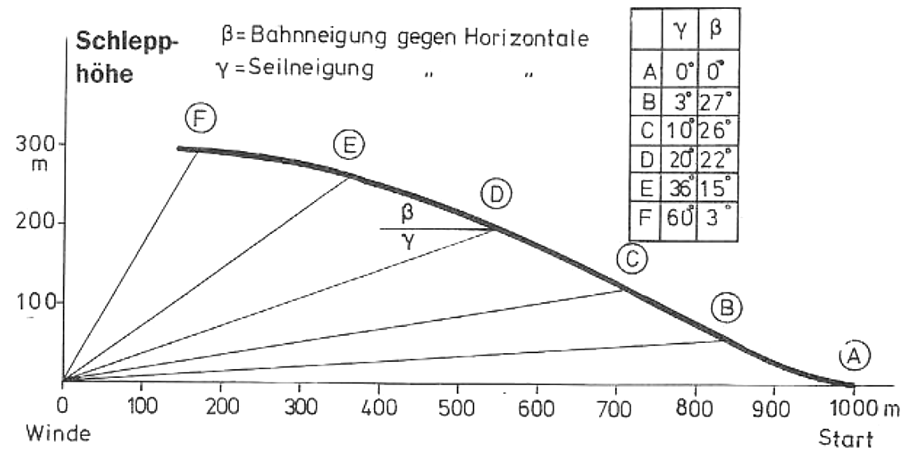
\includegraphics[width=120mm]{Windenstart.png}
		\caption{Höhenverlauf bei Schleppvorgang \cite{PhysikWindenschlepp}}
		\label{fig:HoehenverlaufSchlepp}
	\end{center}
\end{figure}

Es ergibt sich gut ersichtlich eine abgeflachte Kurve am Anfang und am Ende des Schleppvorganges. Sobald sich der Pilot vom Seil getrennt hat, wird das Seil durch einen bereits am Seil befestigten Fallschirm zu Boden geführt und auf der Winde eingezogen. Damit der nächste Pilot starten kann, müssen je nach Windenart unterschiedliche Massnahmen getroffen werden, deshalb werden nachfolgend die Einzugswinde und die Abrollwinde genauer beschrieben.


\textbf{Einzugswindenbetrieb:}
Beim Einzugsbetrieb ist die Winde stationär am Boden befestigt und das Seil wird auf die gewünschte Länge ausgezogen. Bei Startbeginn befindet sich der Pilot gegenüber der Winde einige hundert Meter entfernt. Wärend dem Betrieb wird entsprechend das Seil auf der Winde aufgerollt, respektive der Pilot zur Winde hingezogen. Die Regulierung der Geschwindigkeit erfolgt direkt über die Drehzahl-Einstellung des Motors und darf eine maximale Geschwindigkeit am Gleitschirm von 12m/s erreichen.

\textbf{Abrollwindenbetrieb:}
Beim Abrollwindenbetrieb wird die Winde an einem Auto (Ladefläche bei Pickup) befestigt. Das Auto übernimmt somit bei Betrieb die treibende Kraft und bewegt sich vom Piloten weg. Damit der Pilot, welcher beim Start lediglich einige Meter hinter dem Auto steht, eine Kraft in Horizontalrichtung empfängt und in die Luft gehoben wird, muss die Winde während dem Abrollvorgang bremsen. Die Kraftregulierung erfolgt direkt mit der Bremskraft mit welcher die Winde abgebremst wird. Die theoretisch maximale Kraft wird erreicht, wenn die Winde blockiert wird und sich somit der Pilot gleich schnell vorwärts bewegt wie das voreilende Fahrzeug. Es gilt zu beachten, dass die Bremsung elektrisch erreicht wird und dadurch der Elektromotor nicht exakt auf Drehzahl null herunter gebremst werden kann. Wie bereits erwähnt hat ein Gleitschirm während dem Schleppvorgang gegenüber Wind eine Geschwindigkeit von 10m/s. Optimalerweise fährt der Fahrzeugführende mit einer Vorwärtsgeschwindigkeit, welche bei Windenblockade beim Piloten eine Vorwärtsgeschwindigkeit gegenüber Wind von 12m/s - 15m/s ergeben. Erfahrungsgemäss liegt in den meisten Fällen die Geschwindigkeit des Autos bei rund 50km/h.


\subsection{Anforderungen}\label{subsec:Richtlinien}
Die gesetzlichen Bestimmungen für die gesamte Seilwinde wurden bereits im Pflichtenheft thematisiert und aufgelistet. Nachfolgend werden daher lediglich die für die Auswahl von Motor und Controller, sowie dessen Validierung relevanten Vorschriften aufgeführt. Ausserdem sind auch Anforderungen an Energieversorgung und mechanischen Komponenten wie Seil und Sollbruchstellen kurz erläutert. Für eine detaillierte Erläuterung aller Anforderungen wird auf das technische Pflichtenheft\cite{TechPflichtenheft} verwiesen. Die Liste aus dem Pflichtenheft mit den Anforderungen sind zudem im Anhang \ref{appsec:Anforderungen} hinterlegt.

Durch die elektrische Versorgung des Motors, unterliegt das Projekt der Norm der IEC (International Electrotechnical Commission). Damit die Richtlinien möglichst tief gehalten werden können, fiel der Entschied auf den Kleinspannungsbereich (Spannungsbereich \RM{1} nach IEC 60449), was einer Spannung $U_{DC}<120V_{DC}$ oder $U_{AC}<50V_{AC}$ entspricht. Dies bringt den Vorteil mit sich, dass keine für den Mensch gefährlichen Spannungen auftreten können, was geringere Vorschriften an Isolation, Berührungsschutz und Leitungsführung mit sich bringt.
Die Anforderungen an den Betrieb der Winde gestalten sich durch nachfolgende Parameter. Die Zugkraft der Seilwinde (respektive des Seils) muss eine minimale Zugkraft von 600N erreichen und darf beim Einzelschlepp den Wert von $ 1000N $ nicht überschreiten. Werden zwei Personen gleichzeitig geschleppt (auch Doppelschlepp genannt), darf diese auf maximal $ 1300N $ erhöht werden. Die Zugkraft muss dem Windenführer stets bekannt sein und wird durch eine Kraftanzeige an einem Display erreicht.
Weiter darf während des Schleppvorgangs eine maximale Welligkeit von $\pm 25N$ auftreten. Das bedeutet, dass ein Oszillierender Einzug mit der genannten Kraftamplitude erlaubt ist. Wird der Winde ein Drehmomentsollwert vorgegeben, so darf diese nicht mehr als $\pm 100N$ davon abweichen. Das bedeutet, bei maximaler Zugkraft (im Einzelschlepp) dürfen Werte zwischen $ 900N $ und $ 1100N $ auftreten. Aus Sicherheitsgründen wird die maximale Einzugsgeschwindigkeit begrenzt. Da bei Nullwind eine Einzugsgeschwindigkeit von 10m/s für optimales Steigen sorgt und evt. leichte Rückenwinde während dem Schleppvorgang auftreten können, wurde die Geschwindigkeit des Seil auf maximal $ 12m/s $ gelegt.
Zur Sicherheit des Piloten, muss ein Schleppvorgang jederzeit abgebrochen werden können. Dies kann einerseits durch Leerlauf des Motors oder im schlimmsten Fall durch einen Kappvorgang des Seils erreicht werden. Neben der Kappvorrichtung müssen auch Vorseil, Schleppseil, Verbindungsteile und Reparaturstellen eine minimale Reissfestigkeit von > 4000N erreichen, so wie Sollbruchstellen mit einer Bruchlast von min. 1500N im Soloschlepp und min. 2000N im Doppelschlepp \cite{WindenPruefanweisung}.


Da der Motor primär von Batterien gespiesen wird und diese eine begrenzte Kapazität vorweisen, wurde ein batteriebetriebener Schleppvorgang von minimal fünf Startvorgänge definiert. Ein weiterer Betrieb wird durch einen Hilfsgenerator ermöglicht, welcher lediglich zur Unterstützung der Batterie dient und somit nicht die gesamte Leistung übernimmt. Die Batterien müssen zudem sowohl gegen Tiefen- als auch gegen Überladung geschützt werden.